\section{Projektmanagement}

\subsection{Projektübersicht}
Das Hauptziel dieser Bachelorarbeit...

\subsubsection{Ziele der Projektes}


\subsection{Projektorganisation}
Diese Bachelorarbeit wird von zwei Personen umgesetzt und durch zwei Betreuer überwacht.

\subsubsection{Organisationsstruktur}


\subsection{Management Abläufe}
Für die Umsetzung der Bachelorarbeit stehen insgesamt 14 Wochen und pro Person 360 Stunden zur Verfügung. In einer Woche liegt das Arbeitspensum von 26 Stunden pro Person vor. Das Projekt startet am 17. September 2018 und endet am 21. Dezember 2018.

\subsubsection{Zeitliche Planung}
Die zeitliche Planung, sowie die Verwaltung der Arbeitspakete erfolgte auf Waffle.io. Die Planung wird während dem Projekt laufend aktualisiert und angepasst. Die Arbeitszeiten werden während der Arbeitsausführung mit Toggle erfasst.



\subsubsection{Meilensteine}
Folgende Meilensteine sind für das Projekt definiert:



\subsubsection{Arbeitspakete}
Alle Arbeitspakete werden in Waffle.io erfasst und sind unter folgendem Link ersichtlich:
\href{Waffle.io}{https://waffle.io/night28/HSR\_BA}
\subsubsection{Besprechungen}
Die Besprechungen mit dem Betreuer finden an den nachfolgend aufgelisteten Tagen statt:
\begin{itemize}
	\item jeden Mittwoch zwischen 10.30 - 11.30 Uhr
\end{itemize}

Offene Traktanden und Probleme werden mit dem Betreuer diskutiert. Nach dieser Besprechung wird jeweils in einem Team-Meeting das weitere Vorgehen geplant.


\subsection{Infrastruktur}
Die Organisation der Arbeit und Teammitglieder wird durch folgende Werkzeuge unterstützt:

\begin{figure}[H]
	\centering
	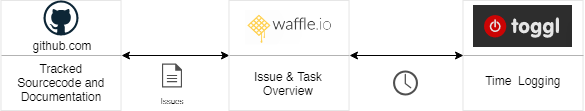
\includegraphics[width=13cm]{img/EingesetzteToolsZurOrganisation.png}
	\caption{Übersicht über die Verknüpfung der eingesetzten Werkzeuge zur internen Organisation.}
	\label{fig:Interne Organisationsstruktur}
\end{figure} 

Unsere Tools sind unter folgenden Links einsehbar:
\paragraph{GitHub} \href{https://github.com/night28/HSR\_BA}{https://github.com/night28/HSR\_BA} 

\paragraph{Waffle.io} \href{https://waffle.io/night28/HSR\_BA}{https://waffle.io/night28/HSR\_BA}

\paragraph{Toggl} \href{https://toggl.com/}{https://toggl.com/}
 
\subsection{Risiko Management}

\subsubsection{Umgang mit Risiken}


\subsubsection{Risiken}


\subsubsection{Eingetretene Risiken}
